% !TEX root = saveliev_physics_general_course_1.tex
%!TEX TS-program = pdflatex
%!TEX encoding = UTF-8 Unicode

%\chapter{HYDRODYNAMICS}\label{chap:9}

\chapter{THUỶ ĐỘNG LỰC HỌC}\label{chap:9}

%\section{Streamlines and Flow Tubes. Flow Continuity}\label{sec:9_1}

\section{Các đường và ống dòng. Tính liên tục của dòng.}\label{sec:9_1}

%Mechanics of continuous media exists in addition to the mechanics of a point particle and the mechanics of a rigid body which we treated in preceding chapters. This science covers hydrodynamics, gas dynamics, the theory of elasticity (some questions of which were dealt with in Secs.~\ref{sec:2_9} and~\ref{sec:3_8}), and a number of other branches of science considering a substance as a continuous medium. Hydrodynamics is the branch of mechanics of continuous media studying the motion of incompressible liquids and their interaction with solids.

Ngoài cơ học chất điểm và cơ học vật rắn mà ta đã nghiên cứu trong các chương trước, còn tồn tại môn cơ học các môi trường liên tục. Ngành khoa học này bao gồm thuỷ động lực học, khí động lực học, lý thuyết đàn hồi (Một số vấn đề của lý thuyết đàn hồi đã được nói đến trong Mục~\ref{sec:2_9} và~\ref{sec:3_8}) và hàng loạt các môn học khác, nghiên cứu chất như một môi trường liên tục. Thuỷ động lực học là một phần của cơ học các môi trường liên tục trong đó người ta nghiên cứu sự chuyển động của các chất lỏng không chịu nén và sự tương tác của các chất lỏng không chịu nén với vật rắn.

%To describe the motion of a liquid, we can set the position of each of its particles as a function of time. This method of description was worked out by J.~Lagrange. But it is also possible to observe separate points of space instead of liquid particles and record the velocity with which separate particles of the liquid pass each given point. The second method is called the Euler method.

Để mô tả chuyển động của chất lỏng, có thể cho vị trí của mỗi hạt chất lỏng như một hàm của thời gian. Cách mô tả như vậy đã được Lagrange nghiên cứu. Nhưng có thể theo dõi không phải các hạt chất lỏng mà là các điểm riêng biệt của không gian và nhận xét vận tốc của các hạt chất lỏng riêng biệt đi qua mỗi điểm này. Phương pháp thứ hai gọi là phương pháp Euler.

%The state of motion of a liquid can be determined by indicating the velocity vector as a function of time for each point of space. The combination of the vectors $\vec{v}$ given for all the points of space forms the so-called \textbf{velocity vector field} that can be depicted as follows. Let us draw lines in a flowing liquid so that a tangent to them at each point coincides in direction with the vector $\vec{v}$ (\fig{9_1}). These lines are called \textbf{streamlines}. We shall agree to draw the streamlines so that their density (characterized by the ratio of the number of lines $\Delta N$ to the magnitude of the area $\Delta S$ at right angles to them through which they pass) is proportional to the magnitude of the velocity at the given place. The pattern of the streamlines will thus permit us to assess not only the direction, but also the magnitude of the 	vector $\vec{v}$ at different points of space: the streamlines will be closer together where the velocity is higher and, conversely, farther apart where the velocity is lower.

Có thể xác định được trạng thái chuyển động của chất lỏng bằng cách chỉ ra cho mỗi điểm của không gian một vector vận tốc như một hàm của thời gian. Tập hợp các vector $\vec{v}$ được cho đối với mọi điểm của không gian sẽ tạo thành cái gọi là \textbf{trường vector vận tốc} mà có thể biểu diễn nó như sau. Ta vẽ trong chất lỏng chuyển động các đường sao cho tiếp tuyến với chúng tại mỗi điểm trùng với phương của vector $\vec{v}$ (\fig{9_1}). Các đường này gọi là các \textbf{đường dòng}. Ta quy ước vẽ các đường dòng sao cho độ dày (được đặc trưng bằng tỷ số của số đường sức từ  $\Delta N$ với độ lớn của diện tích $\Delta S$ vuông góc với chúng mà chúng xuyên qua) của chúng tỷ lệ với độ lớn của vận tốc ở chỗ đã cho. Khi ấy theo bức tranh các đường dòng ta có thể phán đoán không chỉ về hướng mà cả về độ lớn của vector $\vec{v}$ tại các điểm khác nhau của không gian: tại nơi nào vận tốc lớn hơn thì các đường dòng ở đấy sẽ dày hơn, và ngược lại tại nơi vận tốc nhỏ hơn các đường dòng sẽ thưa hơn.

%Since the magnitude and the direction of the vector $\vec{v}$ may change with time at every point, then the pattern of the streamlines may also change continuously. If the velocity vector is constant at each point of space, then the flow is called \textbf{steady}. In steady flow, any particle of a liquid passes a given point of space with the same value of $\vec{v}$. The pattern of the streamlines in steady flow remains unchanged, and the streamlines in this case coincide with the trajectories of the particles.

Vì độ lớn và hướng của vector $\vec{v}$ tại mỗi điểm có thể biến đổi theo thời gian nên chính bức tranh các đường dòng sẽ có thể biến đổi liên tục. Nếu vector vận tốc tại mỗi điểm của không gian vẫn không đổi thì dòng chảy được gọi là dòng chảy ổn định hoặc \textbf{dòng chảy dừng}. Trong dòng chảy dừng, mỗi hạt chất lỏng bất kỳ đi qua một điểm đã cho của không gian với cùng một giá trị của $\vec{v}$. Bức tranh các đường dòng trong dòng chảy dừng vẫn không biến đổi và các đường dòng trong trường hợp này đều trùng với quỹ đạo của các hạt.

\begin{figure}[!htb]
	\begin{center}
		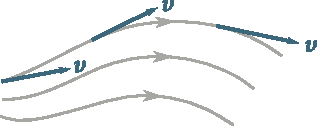
\includegraphics[scale=1.0]{figures/ch_09/fig_9_1.pdf}
		\caption[]{}
		\label{fig:9_1}
	\end{center}
	\vspace{-0.8cm}
\end{figure}

%A portion of a liquid confined by streamlines is called a flow tube. The vector $\vec{v}$, being at each point tangent to a streamline, will also be tangent to the surface of the flow tube. Hence, the particles of the liquid in their motion do not intersect the ``walls'' of the flow tube.

Phần chất lỏng được giới hạn bởi các đường dòng được gọi là một ống dòng. Vector $\vec{v}$ tiếp tuyến với đường dòng tại mỗi điểm sẽ tiếp tuyến với bề mặt ống dòng, do đó các hạt chất lỏng khi chuyển động sẽ không xuyên qua các thành ống dòng.

%Let us take a cross section $S$ of a flow tube (\fig{9_2}) at right angles to the direction of the velocity. We shall assume that the velocity of the liquid particles is the same at all points of this section. During the time $\Delta t$, all the particles whose distance from $S$ at the initial moment did not exceed the value $v\Delta t$ will pass through section $S$. Consequently, a volume of the liquid equal to $Sv$ will pass through section $S$ during the time $\Delta t$, and a volume of the liquid equal to $Sv$ will pass through it in unit time. Let us take a flow tube so thin that at each section of it the velocity may be considered constant. If the liquid is incompressible (\ie, its density is the same everywhere and cannot change), then the amount of liquid between sections $S_1$ and $S_2$ (\fig{9_3}) will remain constant. Hence, it follows that the volumes of liquid flowing in a unit time through sections $S_1$ and $S_2$ must be the same:

Ta hãy lấy một tiết diện ống dòng $S$ vuông góc với hướng của vận tốc (\fig{9_2}). Ta giả thử rằng vận tốc chuyển động của các hạt chất lỏng là như nhau tại mọi điểm của tiết diện này. Trong thời gian $\Delta t$ tất cả các hạt tại thời điểm ban đầu nằm cách $S$ không quá một khoảng $v\Delta t$ sẽ đi qua tiết diện $S$. Do đó trong khoảng thời gian $\Delta t$ thể tích chất lỏng đi qua tiết diện $S$ bằng $Sv\Delta t$, còn trong một đơn vị thời gian thể tích chất lỏng đi qua tiết diện $S$ bằng $Sv$. Ta lấy một ống dòng mảnh đến mức là có thể coi vận tốc là không đổi tại mỗi tiết diện của nó. Nếu chất lỏng là không chịu nén (nghĩa là khối lượng riêng của nó tại mọi nơi là như nhau và không thể bị biến đổi) thì lượng chất lỏng giữa các tiết diện $S_1$ và $S_2$ (\fig{9_3}) sẽ vẫn không thay đổi. Từ đó suy ra rằng các thể tích chất lỏng chảy qua các tiết diện $S_1$ và $S_2$ trong một đơn vị thời gian đều phải như nhau:
\begin{equation*}
	S_1v_1 = S_2v_2
\end{equation*}

\noindent
(ta nhớ rằng các hạt chất lỏng không xuyên qua mặt bên của ống dòng).

%(we remind our reader that the particles of the liquid do not pass through the side surface of a flow tube).

\begin{figure}[!htb]
	\begin{minipage}[t]{0.5\linewidth}
		\begin{center}
			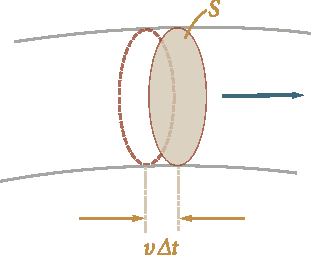
\includegraphics[scale=1.0]{figures/ch_09/fig_9_2.pdf}
			\caption[]{}
			\label{fig:9_2}
		\end{center}
	\end{minipage}
	\hspace{-0.0cm}
	\begin{minipage}[t]{0.5\linewidth}
		\begin{center}
			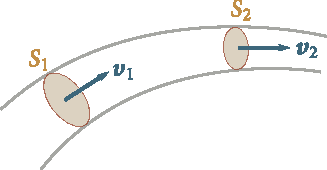
\includegraphics[scale=1.0]{figures/ch_09/fig_9_3.pdf}
			\caption[]{}
			\label{fig:9_3}
		\end{center}
	\end{minipage}
	\vspace{-0.0cm}
\end{figure}

%The above reasoning may be applied to any pair of sections $S_1$ and $S_2$. Consequently, \textit{for an incompressible liquid, the quantity $Sv$ must be the same for any section of the same flow tube}:

Lập luận dẫn ra trên đây được áp dụng cho một cặp tiết diện $S_1$ và $S_2$ bất kỳ. Do đó, \textit{đối với một chất lỏng không chịu nén, đại lượng $Sv$ tại một tiết diện bất kỳ của cùng một ống dòng phải như nhau}:
\begin{equation}\label{eq:9_1}
	Sv = \text{constant}.
\end{equation}

\noindent
%The result obtained forms the content of the theorem on \textbf{flow continuity}.

Kết quả mà ta thu được là nội dung của định lý về \textbf{tính liên tục của dòng}.

%It can be seen from \eqn{9_1} that when a flow tube has a varying section the particles of an incompressible liquid will move with acceleration. In a horizontal flow tube (\fig{9_4}), this acceleration can be due only to the lack of constancy of the pressure along the axis of the tube---at places where the velocity is smaller, the pressure must be greater, and vice versa. The quantitative relation between the flow velocity and the pressure will be established in the following section.

Từ \eqn{9_1} suy ra rằng khi tiết diện của ống dòng thay đổi, các hạt của chất lỏng không chịu được nén sẽ chuyển động có gia tốc. Trong một ống dòng nằm ngang (\fig{9_4}) gia tốc này có thể được gây ra chỉ bởi sự thay đổi áp suất dọc theo trục ống, nghĩa là tại những chỗ mà vận tốc nhỏ hơn thì áp suất phải lớn hơn và ngược lại. Sự liên hệ định lượng giữa vận tốc chảy và áp suất sẽ được thiết lập ở mục sau.

%The theorem on flow continuity can be applied to real liquids and even to gases when their compressibility may be disregarded. The relevant calculations show that when fluids flow with velocities lower than the speed of sound, they may be considered incompressible with a sufficient degree of accuracy.

Định lý về tính liên tục của dòng được áp dụng cho các chất lỏng thực và ngay cả cho các chất khí nếu như có thể bỏ qua được tính chịu nén của chúng. Phép tính toán thích hợp chứng tỏ rằng khi các chất lỏng và các chất khí chuyển động với các vận tốc nhỏ hơn vận tốc của âm thì với mức độ đủ chính xác có thể coi chúng là không chịu nén.

\begin{figure}[!htb]
	\begin{center}
		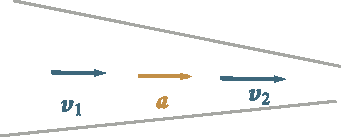
\includegraphics[scale=1.0]{figures/ch_09/fig_9_4.pdf}
		\caption[]{}
		\label{fig:9_4}
	\end{center}
	\vspace{-0.8cm}
\end{figure}

%\section{Bernoulli's Equation}\label{sec:9_2}

\section{Phương trình Bernoulli}\label{sec:9_2}

%When dealing with the motion of liquids, we can often consider that the displacement of some portions of a liquid relative to others is not associated with the appearance of forces of friction. A liquid in which internal friction (viscosity) is completely absent is called \textbf{ideal} (or \textbf{non-viscous}).

Khi xét chuyển động của các chất lỏng, trong nhiều trường hợp có thể coi sự dịch chuyển của các phần này của chất lỏng đối với các phần khác không liên hệ với sự xuất hiện các lực ma sát. Chất lỏng mà trong đó hoàn toàn không có sự ma sát bên trong (sự nhớt) được gọi là \textbf{chất lỏng lý tưởng}.

%Let us separate a flow tube of small cross section (\fig{9_5}) in a steadily flowing ideal liquid. We shall consider the volume of the liquid confined by the ``walls'' of the flow tube and by cross sections $S_1$ and $S_2$ perpendicular to the streamlines. During the time $\Delta t$, this volume will move along the flow tube. Section $S_1$ will move to position $S_1'$ having covered the distance $\Delta l_1$, and section $S_2$ will move to position $S_2'$ having covered the distance $\Delta l_2$. Owing to flow continuity, the shaded volumes will be equal: $\Delta V_1 = \Delta V_2 = \Delta V$.

Ta hãy tách riêng một ống dòng có tiết diện nhỏ trong một chất lỏng lý tưởng chảy dừng (\fig{9_5}). Ta xét thể tích chất lỏng được giới hạn bởi các thành ống dòng và các tiết diện $S_1$ và $S_2$ vuông góc với các đường dòng. Trong thời gian $\Delta t$ thể tích này dịch chuyển dọc theo ống dòng, hơn nữa tiết diện $S_1$ dịch chuyển sang vị trí $S_1'$ bằng cách đi qua quãng đường $\Delta l_1$, tiết diện $S_2$ dịch chuyển sang vị trí $S_2'$ bằng cách đi qua quãng đường $\Delta l_2$. Do tính liên tục của dòng các thể tích gạch gạch sẽ có độ lớn như nhau: $\Delta V_1 = \Delta V_2 = \Delta V$.

\begin{figure}[!htb]
	\begin{center}
		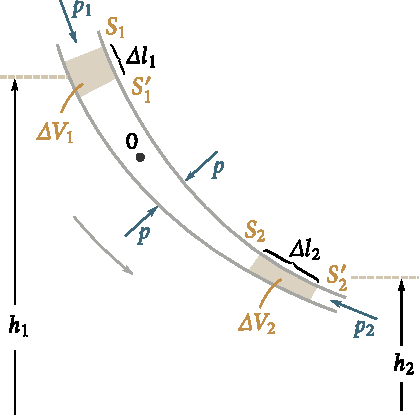
\includegraphics[scale=1.0]{figures/ch_09/fig_9_5.pdf}
		\caption[]{}
		\label{fig:9_5}
	\end{center}
	\vspace{-0.8cm}
\end{figure}

%The energy of each liquid particle consists of its kinetic energy and its potential energy in the field of the Earth's gravitational forces. Owing to the steady nature of the flow, a particle that after the time $\Delta t$ is at any point in the unshaded part of the volume being considered (see, for example, point $0$ in \fig{9_5}) has the same velocity (and, consequently, kinetic energy) as the particle did that was at the same point at the initial moment. Hence, the energy increment $\Delta E$ of the entire volume being considered can be calculated as the difference between the energies of the small shaded volumes $\Delta V_1$ and $\Delta V_2$.

Năng lượng của mỗi hạt chất lỏng bao gồm động năng và thế năng của nó trong trường lực hút của Trái đất. Do tính dừng của dòng chảy, một hạt sau thời gian $\Delta t$ nằm ở một điểm bất kỳ trong các điểm của phần không gạch gạch của thể tích được xét (chẳng hạn, xem điểm  $0$ trên \fig{9_5}) sẽ có cùng vận tốc (do đó, có cùng cả động năng) như vận tốc của hạt nằm ở ngay điểm đó tại thời điểm ban đầu. Do đó có thể tính số gia của năng lượng $\Delta E$ của toàn bộ thể tích được xét như hiệu các năng lượng của các thể tích nhỏ được gạch gạch $\Delta V_1$ và $\Delta V_2$.

%Let us take a flow tube cross section and the lengths $\Delta l$ so small that the same values of the velocity $v$, pressure $p$, and height $h$ can be ascribed to all the points of each of the shaded volumes. Hence, the energy increment can be written as follows:

Ta hãy lấy một tiết diện của ống dòng và đoạn $\Delta l$ nhỏ đến nỗi có thể quy cùng một trị số của vận tốc $v$, của áp suất $p$ và của độ cao $h$ cho tất cả các điểm của mỗi thể tích nhỏ được gạch gạch. Khi đó số gia của năng lượng được viết như sau:

\begin{equation}\label{eq:9_2}
	\Delta E = \left(\frac{\rho\Delta V v_2^2}{2} + \rho\Delta V gh_2\right) - \left(\frac{\rho\Delta V v_1^2}{2} + \rho\Delta V gh_1\right)
\end{equation}

\noindent
%($\rho$ is the density of the liquid).

($\rho$ là khối lượng riêng của chất lỏng).

%Forces of friction are absent in an ideal liquid. Therefore, the energy increment~\eqref{eq:9_2} must equal the work done by the pressure forces on a separated volume. The forces of pressure on the side surface are perpendicular at each point to the direction of motion of the particles to which they are applied, consequently, they do no work. Only the work of the forces applied to sections $S_1$ and $S_2$ differs from zero. This work is

Trong chất lỏng lý tưởng không có các lực ma sát. Do đó số gia của năng lượng~\eqref{eq:9_2} phải bằng công thực hiện bởi các áp lực trên thể tích được tách ra. Các áp lực lên bề mặt bên vuông góc với phương dịch chuyển của các hạt tại mỗi điểm mà chúng đặt vào, do đó chúng không thực hiện công. Chỉ có công của các lực đặt vào các tiết diện $S_1$ và $S_2$ là khác không. Công này sẽ bằng
\begin{equation}\label{eq:9_3}
	A = p_1 S_1 \Delta l_1 - p_2 S_2 \Delta l_2 = (p_1 - p_2)\Delta V.
\end{equation}
%Equating Eqs.~\eqref{eq:9_2} and~\eqref{eq:9_3}, cancelling $\Delta V$, and transferring terms with the same subscripts to the same side of the equation, we get

Cho bằng nhau các biểu thức~\eqref{eq:9_2} và~\eqref{eq:9_3}, giản ước cho $\Delta V$ và chuyển các số hạng có các chỉ số như nhau sang cùng một vế của đẳng thức ta có:
\begin{equation}\label{eq:9_4}
	\frac{\rho v_1^2}{2} + \rho gh_1 + p_1 = \frac{\rho v_2^2}{2} + \rho gh_2 + p_2.
\end{equation}

\noindent
%Sections $S_1$ and $S_2$ were taken absolutely arbitrarily. We can therefore assert that the expression $\rho v_1^2/2+\rho gh+p$ has the same value for any section of the flow tube. In accordance with the assumptions we made in deriving \eqn{9_4}, it becomes quite accurate only when the cross section $S$ tends to zero, \ie, when the flow tube contracts into a streamline. Thus, the quantities $p$, $v$ and $h$ in the left-hand and right-hand sides of \eqn{9_4} should be considered as relating to two arbitrary points of the same streamline.

Các tiết diện $S_1$ và $S_2$ được lấy hoàn toàn tuỳ ý. Do đó có thể khẳng định rằng biểu thức $\rho v_1^2/2+\rho gh+p$ có giá trị như nhau tại mọi tiết diện của ống dòng. Căn cứ vào các giả thuyết mà ta đã đưa ra, cùng với kết luận của nó, \eqn{9_4} trở nên hoàn toàn đúng chỉ khi tiết diện ngang $S$ dần tới không, nghĩa là khi ống dòng thu về đường dòng. Vậy các đại lượng $p$, $v$ và $h$ có mặt ở các vế trái và phải của \eqn{9_4} cần được coi như thuộc về hai điểm tuỳ ý của cùng một đường dòng.

%The result obtained can be formulated as follows: \textit{the condition}

Có thể diễn đạt kết quả mà ta đã thu được như sau: \textit{trong sự chảy dừng của chất lỏng lý tưởng, điều kiện}
\begin{equation}\label{eq:9_5}
	\frac{\rho v^2}{2} + \rho gh + p = \text{constant}
\end{equation}

\noindent
%\textit{is observed in a steadily flowing ideal liquid along any streamline}. Equation~\eqref{eq:9_5}, or \eqn{9_4} equivalent to it, is called \textbf{Bernoulli's equation}, in honour of its discoverer, the Swiss mathematician Daniel~Bernoulli (1700-1782). Although we obtained this equation for an ideal liquid, it is obeyed sufficiently well for real liquids in which the internal friction is not very great.

\textit{được nghiệm đúng dọc theo một đường dòng bất kỳ}. Phương trình~\eqref{eq:9_5} hoặc \eqn{9_4} tương đương với nó được gọi là \textbf{Phương trình Bernoulli}. Mặc dù rằng ta thu được phương trình này đối với chất lỏng lý tưởng nhưng nó cũng thu được nghiệm đúng đối với các chất lỏng thực mà trong đó sự ma sát bên trong là không lớn lắm.

%Equation~\eqref{eq:9_5} acquires the following form for a horizontal streamline:

Đối với một đường dòng nằm ngang điều kiện~\eqref{eq:9_5} có dạng:
\begin{equation*}
	\frac{\rho v_1^2}{2} + p_1 = \frac{\rho v_2^2}{2} + p_2
\end{equation*}

\noindent
%\ie, the pressure is smaller at the points where the velocity is great (this was already shown qualitatively in the preceding section).

nghĩa là áp suất là nhỏ hơn tại những điểm mà ở đó vận tốc là lớn hơn (điều này đã được chứng tỏ một cách định tính trong mục trước).

%The diminishing of the pressure at points where the velocity of a flow is greater underlies the design of a water-jet pump (\fig{9_6}). A water stream is fed into a tube opening to the atmosphere so that the pressure at the outlet from the tube is atmospheric. The tube has a constriction through which the water flows with a higher velocity. As a result, the pressure at this spot is below atmospheric. The same pressure sets in the pump chamber surrounding the tube. The chamber communicates with the tube via an opening in its narrow part. By connecting a vessel to be evacuated to the pump chamber, we can pump the air (or some other gas) out of it to a pressure of the order of \SI{100}{\mmHg}. The evacuated air is entrained by the water stream and carried off into the atmosphere.

Sự làm giảm áp suất tại các điểm mà ở đó vận tốc dòng lớn hơn được đặt làm cơ sở của thiết bị bơm nước (\fig{9_6}). Một dòng nước chảy vào một ống thông ra khí quyển, cho nên ở đầu ra của ống áp suất bằng áp suất khí quyển. Trong ống có chỗ thắt lại, theo đó nước chảy với tốc độ lớn, cho nên áp suất tại chỗ đấy sẽ nhỏ hơn áp suất khí quyển. Chính áp suất đó sẽ được hình thành cả trong buồng của bơm bọc ngoài ống, buồng này thông với ống qua chỗ đứt có mặt tại phần hẹp của ống. Nếu nối thể tích cần bơm với buồng của bơm, có thể hút không khí ra khỏi nó (hoặc một chất khí nào khác) đến áp suất vào cỡ \SI{100}{\mmHg}. Không khí hút đi được dòng nước cuốn theo và đưa vào khí quyển.

\begin{figure}[!htb]
	\begin{center}
		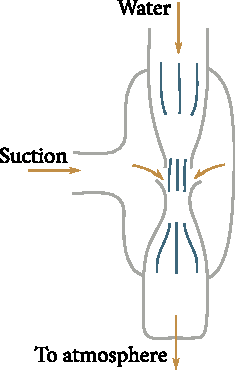
\includegraphics[scale=0.95]{figures/ch_09/fig_9_6.pdf}
		\caption[]{}
		\label{fig:9_6}
	\end{center}
	\vspace{-0.8cm}
\end{figure}

%\section{Flow of a Liquid from a Hole}\label{sec:9_3}

\section{Sự chảy của chất lỏng khỏi một lỗ thủng}\label{sec:9_3}

%Let us apply Bernoulli's equation to the flow of a liquid from a small hole in a wide open vessel. Let us separate in the liquid a flow tube having the open surface of the liquid the vessel as one of its cross sections and the hole through which the liquid flows out\footnote{More exactly, the cross section of the flow emerging front the hole. If special measures are not taken, the section of the Dow will be smaller than the hole.} as the other one (\fig{9_7}). For each of these sections, the velocity and the height above an initial datum level may be considered the same. Consequently, we can apply \eqn{9_4}, obtained on this assumption, to these sections. Further, the pressure in both sections is atmospheric and therefore the same. In addition, the velocity of the open surface in the wide vessel can be assumed to equal zero. With a view to everything said above, \eqn{9_4} can be written in the following form for this case:

Ta hãy áp dụng phương trình Bernoulli cho trường hợp chất lỏng chảy khỏi một lỗ thủng nhỏ trong một bình rộng để hở. Ta hãy tách trong chất lỏng một ống dòng có tiết diện ở phía này là mặt thoáng của chất lỏng trong bình, còn ở phía kia là lỗ thủng theo đó chất lỏng chảy qua\footnote{Chính xác hơn, tiết diện của dòng khí thoát ra khỏi lỗ thủng. Nếu không áp dụng các biện pháp đặc biệt thì tiết diện của dòng sẽ nhỏ hơn lỗ thủng.} (\fig{9_7}). Tại mỗi tiết diện này có thể coi vận tốc và độ cao ở mức ban đầu nào đó đều như nhau, cho nên có thể áp dụng cho nó \eqn{9_4} thu được trong giả thuyết này. Hơn nữa, áp suất tại cả hai tiết diện đều bằng áp suất khí quyển và do đó đều như nhau. Ngoài ra, có thể đặt vận tốc dịch chuyển của mặt thoáng trong một bình rộng bằng không. Nếu kể đến tất cả các điều đã nói, có thể viết \eqn{9_4} phù hợp với trường hợp đã cho dưới dạng
\begin{equation*}
	\rho gh_1 = \frac{\rho v^2}{2} + \rho gh_2
\end{equation*}

\noindent
%where $v$ is the velocity of the liquid flowing from the hole. Cancelling $p$ and introducing $h=h_1-h_2$, \ie, the height of the open surface of the liquid above the hole, we get $v^2/2=gh$, whence

trong đó $v$ là vận tốc chảy thoát khỏi lỗ thủng. Giản ước $p$ và đưa vào $h=h_1-h_2$ là độ cao của mặt thoáng của chất lỏng trên lỗ thủng ta có $v^2/2=gh$, từ đó
\begin{equation}\label{eq:9_6}
	v = (2gh)^{1/2}.
\end{equation}

\noindent
%This formula is known as the \textbf{Torricelli formula}  (after the Italian physicist Evangelista Torricelli, 1608-1647).

Công thức này được gọi là \textbf{công thức Torricelli}

\begin{figure}[!htb]
	\begin{minipage}[t]{0.5\linewidth}
		\begin{center}
			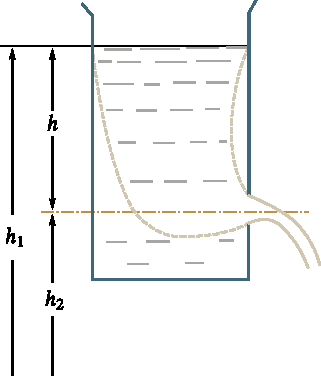
\includegraphics[scale=1.0]{figures/ch_09/fig_9_7.pdf}
			\caption[]{}
			\label{fig:9_7}
		\end{center}
	\end{minipage}
	\hspace{-0.0cm}
	\begin{minipage}[t]{0.5\linewidth}
		\begin{center}
			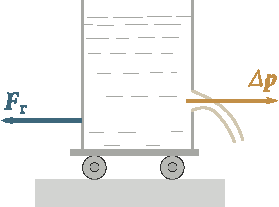
\includegraphics[scale=1.0]{figures/ch_09/fig_9_8.pdf}
			\caption[]{}
			\label{fig:9_8}
		\end{center}
	\end{minipage}
	\vspace{-0.4cm}
\end{figure}

%Thus, the velocity with which a liquid is discharged from a hole at a depth of $h$ under an open surface coincides with the velocity which a body acquires in falling from the height $h$. Do not forget that this result was obtained on the assumption that the liquid is ideal. The discharge velocity will be smaller for real liquids, the difference from the value given by \eqn{9_6} growing with an increasing viscosity of the liquid.

Như vậy, vận tốc chảy thoát của chất lỏng khỏi lỗ thủng đặt ở độ sâu $h$ dưới mặt thoáng trùng với vận tốc của một vật bất kỳ có được khi rơi từ độ cao $h$. Cần nhớ rằng kết quả này có được với giả thiết là chất lỏng là lý tưởng. Đối với các chất lỏng thực vận tốc chảy thoát sẽ nhỏ hơn, hơn nữa nó càng khác giá trị \eqn{9_6} nhiều khi độ nhớt của chất lỏng càng lớn.

%A stream of liquid discharged from a hole in a vessel (\fig{9_8}) carries along with it during the time $\Delta t$ the momentum $\Delta\vec{p}=\rho Sv\vec{v}\Delta t$ ($\rho$ is the density of the liquid, $S$ is the cross-sectional area of the hole, $\vec{v}$ is the discharge velocity of the flow). This momentum is imparted to the discharged liquid by the vessel. According to Newton's third law, the vessel receives a momentum equal to $\Delta\vec{p}$ from the discharged liquid during the time $\Delta t$, \ie, experiences the action of the force

Dòng chất lỏng chảy khỏi lỗ thủng ở bình (\fig{9_8}) trong thời gian $\Delta t$ sẽ mang theo một xung lượng $\Delta K=\rho Sv\vec{v}\Delta t$ ($\rho$ là khối lượng riêng của chất lỏng, $S$ là diện tích lỗ thủng, $\vec{v}$ là vận tốc chảy thoát của dòng). Xung lượng này do bình truyền cho chất lỏng chảy ra. Theo định luật Newton thứ ba, trong thời gian $\Delta t$ bình thu được từ chất lỏng chảy ra một xung lượng bẳng -$\Delta\vec{p}$, nghĩa là chịu tác dụng một lực

\begin{equation}\label{eq:9_7}
	\vec{F}_{\text{r}} = -\frac{\Delta\vec{p}}{\Delta t} = -\rho Sv\vec{v}.
\end{equation}
\noindent

%This force is called the \textbf{reaction of the discharged flow} (or the \textbf{thrust}). If our vessel is placed on a cart, then under the action of the force $\vec{F}_{\text{r}}$ it will start moving in the direction opposite to that of the discharged flow.

Lực này được gọi là \textbf{phản lực của dòng chảy ra}. Nếu đặt bình lên một xe nhỏ thì dưới tác dụng của lực $\vec{F}_{\text{r}}$ nó chuyển động về hướng ngược với hướng của dòng.

%Let us find the value of the force $\vec{F}_{\text{r}}$ using \eqn{9_6} for the discharge velocity of a liquid from a hole:

Ta tìm giá trị của lực $\vec{F}_{\text{r}}$ bằng cách sử dụng biểu thức \eqn{9_6} đối với vận tốc chảy thoát của chất lỏng khỏi lỗ thủng:

\begin{equation}\label{eq:9_8}
	F_{\text{r}} = \rho Sv^2 = 2gh\rho S.
\end{equation}
\noindent

%If, as may seem at first sight, the force $\vec{F}_{\text{r}}$ coincided in magnitude with the force of hydrostatic pressure which the liquid would exert on a plug closing the hole, then $F_{\text{r}}$ would equal $gh\rho S$. The force $\vec{F}_{\text{r}}$ is actually double this value. The explanation is that the motion of the liquid in the vessel appearing when it is discharged leads to redistribution of the pressure, and the pressure near the wall opposite the hole is somewhat greater than near the wall containing the hole.

Nếu như điều thoạt nhìn có thể thấy là lực $\vec{F}_{\text{r}}$ trùng về độ lớn với áp lực thuỷ tĩnh mà chất lỏng có thể tác dụng lên một cái nút đóng vào lỗ thủng, thì $F_{\text{r}}$ sẽ bằng $gh\rho S$. Thật ra, lực $\vec{F}_{\text{r}}$ lớn gấp hai lần. Điều này được giải thích là sự chuyển động của chất lỏng trong bình xuất hiện khi dòng chảy thoát sẽ dẫn tới sự phân bố lại áp suất, thêm vào đó áp suất ở gần thành nằm đối diện với lỗ sẽ hơi lớn hơn áp suất ở gần thành mà tại đó người ta khoét lỗ.

%The operation of jet engines and rockets is based on the reaction or thrust of a discharged gas stream. Reactive motion, not requiring an atmosphere for its accomplishment, is used for flights in outer space.

Hoạt động của các động cơ phản lực và tên lửa dựa trên phản ứng của dòng khí chảy ra. Chuyển động phản lực được sử dụng cho các chuyến bay vào khoảng không vũ trụ, vì để thực hiện nó không cần sự có mặt của khí quyển.

%The outstanding Russian scientist and inventor Konstantin Tsiolkovsky (1857-1935) founded the theory of interplanetary communications. He presented the theory of a rocket's flight and substantiated the possibility of using jet engines for interplanetary flights. In particular, Tsiolkovsky worked out the theory of motion of composite rockets in which each following stage starts functioning after the preceding stage, having completely used up its fuel, separates from the rocket. Tsiolkovsky's ideas were further developed and realized by Soviet scientists and engineers who ensured the leading role of the Soviet Union in the mastering and studying of outer space.

Nhà bác học, nhà phát minh xuất sắc người Nga Konstantin Tsiolkovsky (1857-1935) là người đặt nền móng cho lý thuyết về sự liên lạc giữa các hành tinh. Ông đã đưa ra lý thuyết bay của tên lửa và đã lập luận về khả năng ứng dụng của các máy bay phản lực cho sự liên lạc giữa các hành tinh. Cụ thể là Tsiolkovsky đã vạch ra lý thuyết chuyển động của các tên lửa nhiều tầng, trong đó tầng sau bắt đầu hoạt động sau khi tầng trước bị tách khỏi tên lửa, khi đã tiêu thụ hết nhiên liệu. Các tư tưởng của Tsiolkovsky đã được phát triển về sau và được các nhà bác học và các kỹ sư Xô Viết thực hiện, đảm bảo vai trò tiên phong của Liên Xô trong sự khai thác và nghiên cứu không gian vũ trụ.

%\section{Forces of Internal Friction}\label{sec:9_4}

\section{Các lực nội ma sát}\label{sec:9_4}

%An ideal liquid, i.\ie, one without friction, is an abstraction. Viscosity or internal friction is a property inherent to some extent or other in all real fluids (liquids and gases). Viscosity manifests itself in that motion set up in a fluid gradually stops after the action of the reasons causing the motion is discontinued.

Chất lỏng lý tưởng, nghĩa là chất lỏng không có ma sát, là điều trừu tượng. Độ nhớt hoặc nội ma sát vốn có trong các chất lỏng hoặc chất khí thực ở mức độ nhiều hoặc ít. Độ nhớt được thể hiện ở chỗ sự chuyển động xuất hiện trong chất lỏng hoặc chất khí bị ngừng lại từ từ sau khi các nguyên nhân gây ra chúng đã ngừng tác dụng.

%Let us consider the following experiment to reveal the laws which forces of internal friction obey. Two parallel plates whose linear dimensions considerably exceed the distance $d$ between them (\fig{9_9}) are immersed in a liquid. The bottom plate is held in place, while the top one is brought into motion relative to the bottom one with a certain velocity $\vec{v}_0$. The experiment shows that to move the top plate with a constant velocity $\vec{v}_0$, we have to exert on it a quite definite force $\vec{F}$ that is constant in magnitude. Since the plate receives no acceleration, this signifies that the action of this force is balanced by a force equal to it in magnitude and opposite in direction which is evidently the force of friction acting on the plate when it moves in the liquid. Let us denote it by $\vec{F}_{\text{fr}}$.

Để giải thích quy luật mà các nội lực ma sát tuân theo ta hãy xét thí nghiệm sau đây. Nhúng vào chất lỏng hai bản song song với nhau (\fig{9_9}) có các kích thước dài lớn hơn hẳn khoảng cách $d$ giữa chúng. Bản dưới được giữ nguyên tại chỗ, còn bản trên chuyển động đối với bản dưới với vận tốc $\vec{v}_0$. Thí nghiệm cho thấy là, để bản trên dịch chuyển với vận tốc không đổi $\vec{v}_0$, cần tác dụng lên nó một lực $\vec{F}$ có độ lớn không đổi và hoàn toàn xác định. Một khi bản chưa thu được gia tốc thì có nghĩa là tác dụng của lực này được cân bằng bởi một lực, bằng về độ lớn nhưng ngược chiều với nó mà, rõ ràng, là lực ma sát tác dụng lên bản khi nó chuyển động trong chất lỏng. Ta kí hiệu nó bằng $\vec{F}_{\text{fr}}$.

%By varying the velocity of the plate $\vec{v}_0$, the area of the plates $S$, and the distance $d$ between them, we can find that

Bằng cách thay đổi vận tốc $\vec{v}_0$ của bản, diện tích $S$ của bản và khoảng cách $d$ giữa chúng, có thể thu được là

\begin{equation}\label{eq:9_9}
	F_{\text{fr}} = \eta\frac{v_0}{d}S
\end{equation}
\noindent

%where $\eta$ is a constant of proportionality depending on the nature and state (for instance, the temperature) of the liquid and called the \textbf{coefficient of internal friction} or the \textbf{viscosity} of the liquid (gas). Sometimes the quantity $\eta$ determined from \eqn{9_9} is called the \textbf{dynamic viscosity} as distinct from the kinematic viscosity $\nu$ equal to $\eta/\rho$, where $\rho$ is the density of the fluid---see Sec.~\ref{sec:9_5}.

trong đó $\eta$ là hệ số tỷ lệ phụ thuộc vào bản chất và trạng thái (chẳng hạn, nhiệt độ) của chất lỏng và được gọi là \textbf{hệ số nội ma sát} hoặc là \textbf{hệ số nhớt} hoặc một cách đơn giản là độ nhớt của chất lỏng (của chất khí). Sometimes the quantity $\eta$ determined from \eqn{9_9} is called the \textbf{dynamic viscosity} as distinct from the kinematic viscosity $\nu$ equal to $\eta/\rho$, where $\rho$ is the density of the fluid---see Sec.~\ref{sec:9_5}.

\begin{figure}[!htb]
	\begin{center}
		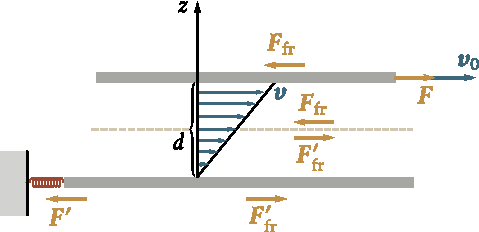
\includegraphics[scale=1.0]{figures/ch_09/fig_9_9.pdf}
		\caption[]{}
		\label{fig:9_9}
	\end{center}
	\vspace{-0.8cm}
\end{figure}

%The bottom plate upon motion of the top one also experiences the action of the force $\vec{F}_{\text{fr}}'$ equal in magnitude to $\vec{F}_{\text{fr}}$. For the bottom plate to remain stationary, the force $\vec{F}_{\text{fr}}$ must be balanced with the aid of the force $\vec{F}'$.

Khi bản trên chuyển động, bản dưới cũng thường chịu tác dụng của lực $\vec{F}_{\text{fr}}'$ về độ lớn bằng $\vec{F}_{\text{fr}}$. Để bản dưới vẫn đứng yên thì cần phải làm cân bằng lực $\vec{F}_{\text{fr}}'$ bằng một lực $\vec{F}'$.

%Thus, when the two plates immersed in the liquid move relative to each other, interaction characterized by the force~\eqref{eq:9_9} appears between them. The plates obviously act on each other through the liquid between the plates, the force of interaction being transmitted from one layer of the liquid to another. If at any place in the gap between the plates we mentally draw a plane parallel to them (see the dash line in \fig{9_9}), then we can assert that the part of the liquid above this plane acts on the part of the liquid under it with the force $\vec{F}_{\text{fr}}$, and the part of the liquid under the plane, in turn, acts on the part above the plane with the force $\vec{F}_{\text{fr}}$, the values of $\vec{F}_{\text{fr}}$ and $\vec{F}_{\text{fr}}'$ being determined by \eqn{9_9}. Thus, \eqn{9_9} determines not only the force of friction acting on the plates, but also the force of friction between the parts of the liquid in contact.

Vậy khi hai bản được nhúng chìm vào chất lỏng chuyển động đối với nhau thì giữa chúng xuất hiện sự tương tác được đặc trưng bằng lực~\eqref{eq:9_9}. Rõ ràng là tác động của các bản với nhau được thực hiện thông qua chất lỏng được chứa đựng giữa các bản, khi truyền từ lớp chất lỏng này sang lớp chất lỏng khác. Nếu tại một vị trí bất kỳ của đường khe ta vẽ một mặt phẳng tưởng tượng song song với các bản (xem đường chấm chấm trên \fig{9_9}), thì có thể khẳng định rằng phần chất lỏng nằm trên mặt phẳng này sẽ tác dụng lên phần chất lỏng nằm dưới mặt phẳng một lực $\vec{F}_{\text{fr}}'$, còn phần chất lỏng nằm dưới mặt phẳng đến lượt mình lại tác dụng lên phần chất lỏng nằm trên mặt phẳng một lực $\vec{F}_{\text{fr}}$, thêm vào đó các trị số của $\vec{F}_{\text{fr}}$ và $\vec{F}_{\text{fr}}'$ đều được xác định bằng \eqn{9_9}. Vậy \eqn{9_9} không chỉ xác định lực ma sát tác dụng lên các bản mà cả lực ma sát giữa các phần chất lỏng tiếp xúc nhau.

%If we study the velocity of the liquid particles in different layers, it will be found to change in the direction $z$ at right angles to the plates (\fig{9_9}) according to a linear law:

Nếu nghiên cứu vận tốc của các hạt chất lỏng tại các lớp khác nhau thì hoá ra là nó bị biến đổi theo phương $z$ vuông góc với các bản (\fig{9_9}) theo định luật tuyến tính:

\begin{equation}\label{eq:9_10}
	v(z) = \frac{v_0}{d}z.
\end{equation}
\noindent

%The liquid particles in direct contact with the plates adhere to them, as it were, and have the same velocity as the plates themselves. By \eqn{9_10},

Các hạt chất lỏng tiếp xúc trực tiếp với các bản như thể dính chặt vào chúng và có cùng vận tốc như vận tốc của chính các bản. Theo \eqn{9_10},

\begin{equation}\label{eq:9_11}
	\left|\diff{v}{z}\right| = \frac{v_0}{d}.
\end{equation}
\noindent

%We have used the magnitude sign for the following reason. If we had fastened the top plate and moved the bottom one (see \fig{9_9}) or had reversed the direction of the $z$-axis, the derivative $\diffin{v}{z}$ would have become negative. The value of $v_0/d$, however, is always positive. Hence, for \eqn{9_11} to hold in any case, we must take the magnitude of $\diffin{v}{z}$.

Ta đặt dấu module vì lý do sau đây. Nếu ta cố định bản trên còn làm chuyển động bản dưới (xem \fig{9_9}), hoặc làm thay đổi hướng của trục $z$ ngược lại thì đạo hàm $\diffin{v}{z}$ có thể trở thành âm. Còn độ lớn của $v_0/d$ bao giờ cũng dương. Do đó để cho \eqn{9_11} đúng trong bất kỳ trường hợp nào thì chỉ cần phải lấy module của $\diffin{v}{z}$.

%Using \eqn{9_11}, we can write \eqn{9_9} as follows:
Nếu sử dụng \eqn{9_11}, có thể cho \eqn{9_9} dạng:

\begin{equation}\label{eq:9_12}
	F_{\text{fr}} = \eta \left|\diff{v}{z}\right| S.
\end{equation}

%This equation determines the magnitude of the force of friction. The quantity $|\diffin{v}{z}|$ shows how fast the velocity changes in the direction of the $z$-axis, and is the magnitude of the gradient of the magnitude of the velocity (if $v$ depends only on $z$, then $\diffinpartial{v}{x}=\diffinpartial{v}{y}=0, \diffinpartial{v}{z}=\diffin{v}{z}$).

Công thức này xác định module của lực ma sát. Độ lớn của $|\diffin{v}{z}|$ chứng tỏ vận tốc bị biến đổi theo phương của trục $z$ nhanh như thế nào và là module của gradient của module vận tốc (nếu $v$ chỉ phụ thuộc vào $z$ thì $\diffinpartial{v}{x}=\diffinpartial{v}{y}=0, \diffinpartial{v}{z}=\diffin{v}{z}$).

%We have obtained \eqn{9_12} for the case when the velocity changes according to a linear law. It was found that this equation also holds for any other law of the change in the velocity from layer to layer. In this case to determine the force of friction between two neighbouring layers, we must take the value of $|\diffin{v}{z}|$ at the place where the imaginary interface between the layers passes.

\eqn{9_12} mà ta thu được đối với trường hợp khi vận tốc được biến đổi theo định luật tuyến tính. Người ta thấy công thức này vẫn đúng cả đối với mọi định luật biến đổi vận tốc từ lớp này sang lớp khác. Trong trường hợp này để xác định lực ma sát giữa hai lớp có chung biên với nhau, cần phải lấy trị số $|\diffin{v}{z}|$ tại vị trí mà ở đó mặt phân cách tưởng tượng giữa các lớp đi qua.

%Everything said in this section relates to all fluids.

Toàn độ điều đã nói trong mục này không chỉ đối với chất lỏng mà cả đối với chất khí.

%The unit of viscosity in the SI system is the viscosity at which the gradient of the velocity with a magnitude of \SI{1}{\metre\per\second} per \si{\metre} leads to the appearance of a force of internal friction of \SI{1}{\newton} per \si{\metre\squared} of surface of contact of the layers. This unit is called the \textbf{pascal-second} (\si{\pascal\second})\footnote{The pascal is the name given to the unit of pressure in the SI system ($\SI{1}{\pascal}=\SI{1}{\newton\per\metre\squared}$).}.

Đơn vị độ nhớt trong hệ SI là độ nhớt mà gradient vận tốc có module bằng \SI{1}{\metre\per\second} trên \SI{1}{\metre}, dẫn tới sự xuất hiện nội lực ma sát là \SI{1}{\newton} trên \SI{1}{\metre\squared} bề mặt tiếp xúc của các lớp. Đơn vị này được gọi là \textbf{pascal-giây} (\si{\pascal\second})\footnote{Đơn vị áp suất trong hệ SI được gọi là pascal ($\SI{1}{\pascal}=\SI{1}{\newton\per\metre\squared}$).}.

%The unit of viscosity in the cgs system is the poise (\si{\poise}) equal to the viscosity at which the gradient of the velocity with a magnitude of \SI{1}{\centi\metre\per\second} per \si{\centi\metre} leads to the appearance of a force of internal friction of \SI{1}{\dyne} per \si{\centi\metre\squared} of surface of contact of the layers. The unit equal to \SI{e-6}{\poise} is called the micropoise (\si{\micro\poise}). The poise and the pascal-second are related as follows:

Trong hệ CGS đơn vị độ nhớt là poise (\si{\poise}) bằng độ nhớt mà gradient vận tốc có module  bằng \SI{1}{\centi\metre\per\second} trên \SI{1}{\centi\metre}, dẫn tới sự xuất hiện lực nội ma sát là \SI{1}{\dyne} trên \SI{1}{\centi\metre\squared} bề mặt tiếp xúc của các lớp. Đơn vị bằng \SI{e-6}{\poise} được gọi là micropoise (\si{\micro\poise}). Giữa poise và pascal-giây có hệ thức:

\begin{equation*}
	\SI{1}{\pascal\second} = \SI{10}{\poise}
\end{equation*}

%The viscosity depends on the temperature. The nature of this dependence appreciably differs for liquids and gases. The viscosity of liquids greatly diminishes with increasing temperature. The viscosity of gases, on the contrary, grows with increasing temperature. The difference in the behaviour of $\eta$ with changes in the temperature points to the difference in the mechanism of internal friction in liquids and gases.

Hệ số nhớt phụ thuộc vào nhiệt độ, thêm vào đó tính chất của sự phụ thuộc này là khác nhau một cách cơ bản đối với các chất lỏng và các chất khí. Ở các chất lỏng, hệ số nhớt sẽ giảm mạnh với sự tăng nhiệt độ. Ở các chất khí, ngược lại, hệ số nhớt tăng cùng với nhiệt độ. Sự khác nhau về tính chất của hành trạng của $\eta$ khi nhiệt độ biến đổi chỉ ra sự khác nhau về cơ chế của nội ma sát trong chất lỏng và chất khí.

%\section{Laminar and Turbulent Flows}\label{sec:9_5}

\section{Dòng chảy thành lớp và dòng chảy rối}\label{sec:9_5}

%Two kinds of flow of a liquid (or gas) are observed. In some cases, the liquid separates, as it were, into layers that slide relative to one another without mixing. Such flow is called \textbf{laminar} (from the Latin word ``lamina'' meaning plate or strip). If we introduce a coloured stream into a laminar flow, it is retained without being washed out over the entire length of the flow because the liquid particles in a laminar flow do not pass over from one layer to another. A laminar flow is steady.

Người ta quan sát hai dạng chảy của chất lỏng (hoặc chất khí). Trong trường hợp này chất lỏng như thể được tách thành các lớp trượt trên nhau chứ không bị dịch chuyển. Sự chảy như thế được gọi là \textbf{dòng chảy thành lớp} (chữ Latin "lamina" có nghĩa là lớp, dải). Nếu đưa vào dòng chảy thành lớp một tia có màu thì tia được giữ nguyên, không bị toè ra trên toàn độ dài của dòng, vì các hạt chất lỏng trong dòng chảy thành lớp không chuyển từ lớp này sang lớp khác. Dòng chảy thành lớp là dòng chảy dừng.

%With an increase in the velocity or cross-sectional dimensions of a flow, its nature changes quite appreciably. Vigorous stirring of the liquid appears. Such a flow is called \textbf{turbulent}. In a turbulent flow, the velocity of the particles at each given place constantly changes chaotically---the flow is not steady. If we introduce a coloured stream into a turbulent flow, already at a small distance from the place of its introduction the coloured liquid will be uniformly distributed over the entire cross section of the flow.

Khi tăng vận tốc hoặc các kích thước ngang của dòng, tính chất của dòng sẽ bị biến đổi một cách cơ bản. Sự pha trộn chất lỏng một cách mạnh mẽ xuất hiện. Dòng chảy như vậy được gọi là \textbf{dòng chảy rối}. Trong dòng chảy rối, vận tốc của các hạt tại mỗi vị trí đã cho luôn luôn bị biến đổi một cách hỗn loạn, nghĩa là dòng chảy không dừng. Nếu đưa vào dòng chảy rối một tia màu đỏ, thì chất lỏng màu đỏ được phân bố dều theo toàn tiết diện của dòng tại một khoảng cách không lớn kể từ chỗ đưa nó vào.

%The British scientist Osborne Reynolds (1842-1912) established that the nature of a flow depends on the value of the dimensionless quantity

Nhà bác học người Anh Osborne Reynolds (1842-1912) đã thiết lập được rằng, tính chất của dòng chảy phụ thuộc vào giá trị của một đại lượng không thứ nguyên

\begin{equation}\label{eq:9_13}
	\reynolds = \frac{\rho n l}{\eta}
\end{equation}
\noindent

%where $\rho$ is the density of the liquid (or gas), $v$ is the average flow velocity (over the cross section of the pipe), $\eta$ is the viscosity of the liquid and $l$ is the dimension characterizing the cross section, for example, the side of the square with a square cross section, the radius or diameter with a round section, etc.

trong đó $\rho$ là khối lượng riêng của chất lỏng (hoặc chất khí) $v$ là vận tốc trung bình (theo tiết diện của ống), $\eta$ là hệ số nhớt của chất lỏng, $l$ là kích thước đặc trưng cho tiết diện ngang, chẳng hạn cạnh của hình vuông ở tiết diện vuông, bán kính hoặc đường kính ở tiết diện tròn, v.v...

%The quantity $\reynolds$ is called the \textbf{Reynolds number}. At small values of the Reynolds number, laminar flow is observed. Beginning from a certain definite value of Re called the critical one, the flow acquires a turbulent nature. If for a round pipe we take its radius $r$ as the characteristic dimension, then the critical value of the Reynolds number (which in this case has the form $\reynolds=\rho vr/\eta$) equals\footnote{It is obvious that if we take the diameter of the pipe instead of its radius as the quantity $l$, we must double the critical value of $\reynolds$.} approximately \num{1000}. The Reynolds number includes the ratio of two quantities depending on the properties of a liquid-the density $\rho$ and the viscosity $\eta$. The ratio

Đại lượng $\reynolds$ được gọi là \textbf{số Reynolds}. Khi các giá trị của số Reynolds nhỏ, ta quan sát được dòng chảy thành lớp. Bắt đầu từ một giá trị nhất định nào đó của Re được gọi là giá trị tới hạn, dòng chảy sẽ có tính chất rối loạn. Nếu lấy bán kính $r$ của một ống tròn làm kích thước đặc trưng cho nó thì trị số tới hạn của số Reynolds (mà trong trường hợp này có dạng $\reynolds=\rho vr/\eta$) là bằng \footnote{Rõ ràng rằng, khi lấy $l$ không phải là bán kính mà là đường kính của ống, ta phải làm tăng giá trị tới hạn $\reynolds$ lên 2 lần.} khoảng \num{1000}. Hai đại lượng phụ thuộc vào các tính chất của chất lỏng là khối lượng riêng $\rho$ và hệ số nhớt $\eta$ tham gia vào số Reynolds dưới dạng một tỉ số. Tỉ số

\begin{equation}\label{eq:9_14}
	\nu = \frac{\eta}{\rho}
\end{equation}
\noindent

%is called the \textbf{kinematic viscosity}. In contrast to $\nu$, the quantity $\eta$ is known as the \textbf{dynamic viscosity}. Using the kinematic viscosity, we can write the Reynolds number as follows:

được gọi là \textbf{độ nhớt động học}, khác với $\nu$, đại lượng $\eta$ được gọi là \textbf{độ nhớt động lực học}. Khi sử dụng độ nhớt động học, có thể cho số Reynolds dạng sau:

\begin{equation}\label{eq:9_15}
	\reynolds = \frac{vl}{\nu}
\end{equation}
\noindent

%The Reynolds number can be used as a dimensionless or similarity number for the flow of liquids in pipes, channels, etc. The nature of the flow of different liquids (or gases) in pipes of different cross sections will be absolutely the same if the same value of $\reynolds$ corresponds to each flow.

Số Reynolds có thể dùng làm tiêu chuẩn của sự đồng dạng đối với dòng chảy của các chất lỏng trong các ống, các kênh, v.v... Tính chất của dòng chảy của các chất lỏng (hoặc các chất khí) khác nhau trong các ống có các tiết diện khác nhau sẽ hoàn toàn như nhau nếu mỗi sự chảy ứng với cùng một giá trị $\reynolds$.

%\section{Flow of a Liquid in a Round Pipe}\label{sec:9_6}

\section{Dòng chất lỏng trong ống tròn}\label{sec:9_6}

%When a liquid flows through a round pipe, the velocity is zero at the pipe walls and maximum at its axis. Assuming the flow to be laminar, let us find the law of the change in the velocity with the distance $r$ from the pipe axis.

Khi chất lỏng chuyển động trong một ống tròn thì vận tốc bằng không ở thành ống và cực đại trên trục của ống. Giả thiết sự chảy là dòng chảy thành lớp, ta hãy tìm định luật biến đổi vận tốc với khoảng cách $r$ kể từ trục của ống. 

\begin{figure}[!htb]
	\begin{center}
		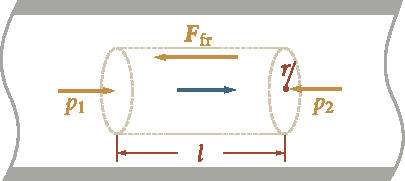
\includegraphics[scale=1.0]{figures/ch_09/fig_9_10.pdf}
		\caption[]{}
		\label{fig:9_10}
	\end{center}
	\vspace{-0.8cm}
\end{figure}

%Let us separate an imaginary cylindrical volume of the liquid of radius $r$ and length $l$ (\fig{9_10}). Upon steady flow in a pipe of constant cross section, the velocities of all the particles of the liquid remain unchanged. Hence, the sum of the external forces applied to any volume of the liquid is zero. The bases of the cylindrical volume being considered experience forces of pressure whose sum is $(p_1-p_2)\pi r^2$. This force acts in the direction of motion of the liquid. In addition, the side surface of the cylinder experiences a force of friction equal to $\eta|\diffin{v}{r}|2\pi rl$ (we have in view the value of $\diffin{v}{r}$ at the distance $r$ from the pipe axis). The condition for steady flow has the form

Ta hãy tách riêng một thể tích chất lỏng hình trụ tưởng tượng có bán kính $r$ và độ dài $l$ (\fig{9_10}). Với dòng chảy dừng trong một ống có tiết diện không đổi, các vận tốc của mọi hạt chất lỏng là không thay đổi. Do đó tổng các ngoại lực đặt vào bất kỳ một thể tích chất lỏng nào là bằng không. Các áp lực có tổng bằng $(p_1-p_2)\pi r^2$ tác dụng lên các đáy của thể tích hình trụ được xét.  Lực này tác dụng theo hướng chuyển động của chất lỏng. Ngoài ra, lực ma sat bằng $\eta|\diffin{v}{r}|2\pi rl$ (khi lưu ý tới giá trị $\diffin{v}{r}$ tại khoảng cách $r$ kể từ trục của ống) tác dụng lên mặt bên của hình trụ. Điều kiện dừng có dạng

\begin{equation}\label{eq:9_16}
	(p_1 - p_2)\pi r^2 = \eta|\diff{v}{r}|2\pi rl.
\end{equation}

%The velocity diminishes with an increasing distance from the pipe axis. Consequently, $\diffin{v}{r}$ is negative, and $|\diffin{v}{r}|=-\diffin{v}{r}$. Taking this into account, we shall transform \eqn{9_16} as follows:

Vận tốc giảm theo khoảng cách kể từ trục của ống. Do đó $\diffin{v}{r}$ là âm và $|\diffin{v}{r}|=-\diffin{v}{r}$. Nếu để ý đến điều này ta biến đổi hệ thức \eqn{9_16} như sau:

\begin{equation*}
	- \diff{v}{r} = \frac{(p_1 - p_2)r}{2\eta l}.
\end{equation*}
\noindent

%Separating the variables, we get
Bằng cách tách các biến số ta thu được phương trình

\begin{equation*}
	\deriv{v} = -\frac{(p_1 - p_2)}{2\eta l}r\,\deriv{r}
\end{equation*}
\noindent

%Integration yields
Lấy tích phân ta được

\begin{equation}\label{eq:9_17}
	v = -\frac{(p_1 - p_2)}{4\eta l}r^2 + C
\end{equation}
\noindent

%The integration constant must be selected so that the velocity will vanish at the pipe walls, \ie, with $r=R$ ($R$ is the pipe radius). From this condition

Cần phải chọn hằng số tích phân sao cho vận tốc triệt tiêu tại các thành ống, nghĩa là khi $r=R$ ($R$ là bán kính của ống). Từ điều kiện này

\begin{equation*}
	C = \frac{(p_1 - p_2)}{4\eta l}R^2.
\end{equation*}
\noindent

%Introduction of the value of $C$ in \eqn{9_17} gives
Thế các giá trị của $C$ vào \eqn{9_17}, sẽ dẫn tới công thức

\begin{equation}\label{eq:9_18}
	v(r) = \frac{(p_1 - p_2)}{4\eta l}\left(R^2 - r^2\right) = \frac{(p_1 - p_2)}{4\eta l}R^2\left(1 - \frac{r^2}{R^2}\right)
\end{equation}
\noindent

%The value of the velocity along the axis of the pipe is
Giá trị của vận tốc trên trục ống bằng

\begin{equation}\label{eq:9_19}
	v_0 = v(0) = \frac{(p_1 - p_2)}{4\eta l}R^2
\end{equation}
\noindent

%By using this equation in \eqn{9_18}, we can obtain
Nếu để ý đến điều đó, có thể cho công thức \eqn{9_18} dạng

\begin{equation}\label{eq:9_20}
	v(r) = v_0 \left(1 - \frac{r^2}{R^2}\right)
\end{equation}
\noindent

%Thus, with laminar flow, the velocity changes with an increasing distance from the axis of a pipe according to a parabolic law (\fig{9_11}).

Vậy trong dòng chảy thành lớp vận tốc biến đổi với khoảng cách kể từ trục ống theo định luật parabol (\fig{9_11}).

%With turbulent flow, the velocity at each point changes chaotically. With constant external conditions, the average (in time) velocity at each point of the cross section of a pipe is constant. The profile of the average velocities in turbulent flow is shown in \fig{9_12}. The velocity changes near the walls of a pipe at a much greater rate than in laminar flow. In the remaining part of the cross section, the change in the velocity is smaller.

Trong dòng chảy rối vận tốc tại mỗi điểm bị biến đổi một cách hỗn loạn. Với những điều kiện bên ngoài không đổi, vận tốc trung bình (theo thời gian) tại mỗi điểm của tiết diện ống là không đổi. Mặt cắt của các vận tốc trung bình trong dòng chảy rối được biểu diễn trên \fig{9_12}. Gần các thành ống vận tốc bị biến đổi mạnh hơn nhiều so với trong dòng chảy thành lớp, còn ngay trong các phần còn lại của tiết diện vận tốc bị biến đổi ít hơn.

\begin{figure}[!htb]
	\begin{minipage}[t]{0.5\linewidth}
		\begin{center}
			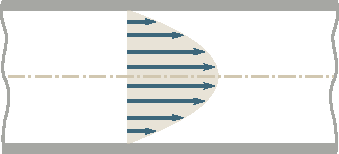
\includegraphics[scale=1.0]{figures/ch_09/fig_9_11.pdf}
			\caption[]{}
			\label{fig:9_11}
		\end{center}
	\end{minipage}
	\hspace{-0.0cm}
	\begin{minipage}[t]{0.5\linewidth}
		\begin{center}
			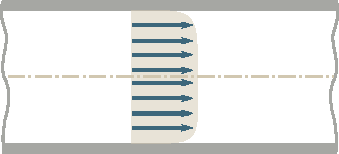
\includegraphics[scale=1.0]{figures/ch_09/fig_9_12.pdf}
			\caption[]{}
			\label{fig:9_12}
		\end{center}
	\end{minipage}
	\vspace{-0.4cm}
\end{figure}

%Assuming the flow to be laminar, let us calculate the rate of flow of the liquid $Q$, \ie, the volume of liquid flowing through the cross section of a pipe in unit time. Let us divide the cross section of the pipe into rings with a width of $\deriv{r}$ (\fig{9_13}). In one second, a volume of liquid equal to the product of the ring area $2\pi r\,\deriv{r}$ and the velocity of the flow at the points at a distance of $r$  from the pipe axis will pass through a ring of radius $r$. With a view to \eqn{9_20} we get

Giả thử dòng chảy là dòng chảy thành lớp, ta hãy tính thông lượng chất lỏng $Q$, nghĩa là thể tích chất lỏng chảy qua một tiết diện ngang của ống trong một đơn vị thời gian. Ta phân tích một tiết diện ngang của ống thành một vòng khuyên có bè rộng $\deriv{r}$ (\fig{9_13}). Thể tích chất lỏng đi qua vòng khuyên có bán kính $r$ trong một giây bằng tích diện tích của vòng $2\pi r\,\deriv{r}$ với vận tốc chảy tại các điểm ở cách trục của ống một khoảng $r$. Chú ý tới \eqn{9_20} ta thu được

\begin{equation}\label{eq:9_21}
	\deriv{Q} = v_0 \left(1 - \frac{r^2}{R^2}\right) 2\pi r\,\deriv{r}
\end{equation}
\noindent

%To obtain the rate of flow $Q$, we must integrate \eqn{9_21} with respect to $r$ within the limits from zero to $R$:

Để thu được thông lượng $Q$ cần phải lấy tích phân biểu thức \eqn{9_21} theo $r$ trong phạm vi từ không đến $R$:

\begin{equation}\label{eq:9_22}
	Q = \int_{0}^{R} v_0 \left(1 - \frac{r^2}{R^2}\right) 2\pi r\,\deriv{r} = \frac{1}{2}\pi R^2 v_0 = \frac{1}{2}Sv_0
\end{equation}
\noindent

%($S$ is the cross-sectional area of the pipe). Inspection of \eqn{9_22} shows that in a laminar flow the average value of the velocity (over the cross section) is half the value of the velocity at the axis of the pipe.

($S$ là diện tích tiết diện của ống). Từ \eqn{9_22} suy ra rằng trong dòng chảy thành lớp giá trị trung bình (theo tiết diện) của vận tốc bằng nửa giá trị của vận tốc trên trục ống.

\begin{figure}[!htb]
	\begin{center}
		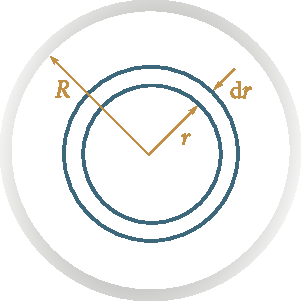
\includegraphics[scale=0.95]{figures/ch_09/fig_9_13.pdf}
		\caption[]{}
		\label{fig:9_13}
	\end{center}
	\vspace{-0.8cm}
\end{figure}

%Substituting in \eqn{9_22} the value for $v_0$ from \eqn{9_19}, we get the following formula for the rate of flow:

Thay \eqn{9_19} đối với $v_0$ vào \eqn{9_22} ta thu được công thức đối với thông lượng

\begin{equation}\label{eq:9_23}
	Q = \frac{(p_1 - p_2)\pi R^4}{8\eta l}
\end{equation}
\noindent

%This formula is called the \textbf{Poiseuille formula}. According to it, the flow of a liquid is proportional to the pressure drop per unit pipe length, to the fourth power of the pipe radius, and is inversely proportional to the viscosity of the liquid. It must be remembered that the Poiseuille formula may be applied only for a laminar flow.

Công thức này được gọi là \textbf{công thức Poiseuille}. Theo \eqn{9_23} thông lượng chất lỏng tỷ lệ với sự sụt áp trên một đơn vị độ dài của ống, tỷ lên với luỹ thừa bậc bốn của bán kính và tỷ lệ nghịch với hệ số nhớt của chất lỏng. Ta nhớ rằng công thức Poiseuille chỉ được áp dụng với dòng chảy thành lớp.

%Formula~\eqref{eq:9_23} is used to determine the viscosity of liquids. By passing a liquid through a capillary of known radius and measuring the pressure drop and the rate of flow $Q$, we can find $\eta$.

Hệ thức~\eqref{eq:9_23} được sử dụng để xác định độ nhớt của chất lỏng. Cho chất lỏng đi qua một ống mao dẫn có bán kính đã biết và đo độ sự sụt áp và thông lượng $Q$, có thể tìm được $\eta$.

%\section{Motion of Bodies in Fluids}\label{sec:9_7}

\section{Chuyển động của vật trong chất lỏng và chất khí}\label{sec:9_7}

%Forces whose resultant will be designated by the symbol $\vec{R}$ (\fig{9_14}) act on a body upon its motion in a fluid\footnote{We shall note that with a constant velocity of a body relative to a fluid the force acting on the body, according to Galileo's principle of relativity, will be the same as when the fluid is moving with the same velocity relative to the stationary body. Figure~\ref{fig:9_14} corresponds to the latter case.}. The force $\vec{R}$ can be resolved into two components, of which $\vec{Q}$ is directed opposite to the motion of the body (or in the direction of the flow advancing onto the body), and $\vec{P}$ at right angles to this direction. The components $\vec{Q}$ and $\vec{P}$ are called the \textbf{drag} (or \textbf{head resistance}) and the \textbf{lift} (or \textbf{lifting force}), respectively. It is obvious that only a drag can act on a body that is symmetrical relative to the direction of motion, while the lift in this case will vanish.

Khi vật chuyển động trong chất lỏng hoặc chất khí\footnote{Chú ý rằng khi vật chuyển động đối với chất lỏng với vận tốc không đổi, lực tác dụng lên vật theo nguyên lý tương đối Galileo cũng giống như trong trường hợp chất lỏng chuyển động với cùng vận tốc đối với vật đứng yên. Hình~\ref{fig:9_14} ứng với trường hợp cuối.}, nó chịu tác dụng của các lực mà ta ký hiệu hợp lực của chúng bằng chữ $\vec{R}$ (\fig{9_14}). Có thể phân tích lực $\vec{R}$ thành hai thành phần mà một trong chúng là $\vec{Q}$ hướng về phía ngược với chuyển động của vật (hoặc về phía chuyển động của dòng thổi đến vật) còn thành phần thứ hai $\vec{P}$ vuông góc với phương này. Các thành phần $\vec{Q}$ và $\vec{P}$ lần lượt được gọi là \textbf{lực cản chính diện} và \textbf{lực nâng}. Rõ ràng là lực cản chính diện chỉ có thể tác dụng lên vật đối xứng với phương chuyển động, còn lực nâng trong trường hợp này sẽ bằng không.

\begin{figure}[!htb]
	\begin{minipage}[t]{0.4\linewidth}
		\begin{center}
			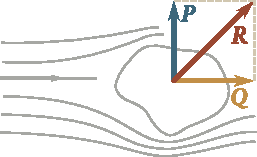
\includegraphics[scale=1.0]{figures/ch_09/fig_9_14.pdf}
			\caption[]{}
			\label{fig:9_14}
		\end{center}
	\end{minipage}
	\hspace{-0.0cm}
	\begin{minipage}[t]{0.6\linewidth}
		\begin{center}
			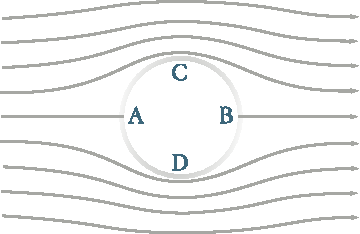
\includegraphics[scale=1.0]{figures/ch_09/fig_9_15.pdf}
			\caption[]{}
			\label{fig:9_15}
		\end{center}
	\end{minipage}
	\vspace{-0.4cm}
\end{figure}

%Calculations show that the uniform motion of bodies in an ideal fluid should occur without drag. Having no viscosity, an ideal fluid should slide freely over the surface of a body, flowing completely around it. Figure~\ref{fig:9_15} shows the streamlines when an ideal fluid flows around a very long (``infinite'') cylinder. Owing to complete flowing around the cylinder, the pattern of the streamlines is absolutely symmetrical both relative to the straight line passing through points A and B and relative to the straight line passing through points C and D. Hence, the pressure near points A and B will be the same (and greater than in an undisturbed flow because the velocity near these points is lower). The pressure near points C and D will also be the same (and lower than in an undisturbed flow because the velocity near these points is higher). Consequently, the resultant force of the pressure on the surface of the cylinder (which in the absence of viscosity could set up a drag) will evidently vanish. The same result is also obtained for bodies of a different shape.

Như các tính toán chứng tỏ, trong chất lỏng lý tưởng, chuyển động đều của các vật phải được xảy ra mà không có lực cản chính diện. Khi không có độ nhớt, chất lỏng lý tưởng phải trượt tự do theo bề mặt của vật bằng cách hoàn toàn chảy quanh vật. Trên hình~\ref{fig:9_15} người ta vẽ các đường dòng khi chất lỏng chảy quanh một hình trụ rất dài (``dài vô tận''). Do chảy quanh toàn bộ nên bức tranh các đường dòng là hoàn toàn đối xứng đối với đường thẳng đi qua điểm A và B cũng như đối với các đường thẳng đi qua các điểm C và D. Do đó áp suất ở gần các điểm A và B sẽ là như nhau (và lớn hơn ở dòng không bị nhiễu loạn, vì vận tốc ở gần các điểm này nhỏ hơn); cũng đúng như vậy, áp suất ở gần các điểm C và D cũng sẽ như nhau (và nhỏ hơn ở dòng không bị nhiễu loạn vì vận tốc gần các điểm này lớn hơn). Do đó hợp lực của các áp lực lên bề mặt hình trụ (mà nó có thể gây ra một lực cản chính diện khi không có độ nhớt), rõ ràng, sẽ bằng không. Người ta thu được một kết quả như vậy đối với các vật có dạng khác.

%Other phenomena are encountered when a body moves in a viscous fluid. In this case, a very thin layer of the fluid adheres to the body's surface and moves together with it as a single whole, carrying along the following layers owing to friction. The velocity of the layers diminishes with an increasing distance from the body's surface and, finally, at a certain distance from the surface the fluid is virtually undisturbed by the motion of the body. The body is thus surrounded by a layer of the fluid in which there is a velocity gradient. This layer is called the \textbf{boundary} one. Friction forces act in it which in the long run are applied to the body and lead to the appearance of a drag. But matters are not exhausted here. The presence of a boundary layer radically changes the nature of the flow of a fluid around a body. Complete flowing around becomes impossible. The action of the friction forces in the surface layer causes the flow to break away from the body's surface. The result is the appearance of eddies behind the body (see \fig{9_16} showing the flow of a viscous fluid around a cylinder). The eddies are carried away by the flow and gradually attenuate owing to friction. The energy of the eddies is spent for heating the fluid. The pressure in the eddy region formed behind the body is lowered. Consequently, the resultant of the pressure forces will differ from zero, this leading in turn to a drag.

Các hiện tượng sẽ xảy ra khác đi khi vật chuyển động trong chất lỏng có tính nhớt. Trong trường hợp này một lớp rất mỏng chất lỏng sẽ dính vào bề mặt của vật và chuyển động với vật như một toàn thể bằng cách cuốn theo các lớp tiếp theo do ma sát. Trong khi ra xa khỏi bề mặt của vật, vận tốc của các lớp đều trở nên nhỏ hơn, và cuối cùng tại một khoảng cách nào đó kể từ bề mặt, thực tế chất lỏng không bị nhiễu loạn bởi chuyển động của vật. Vậy vật được bao quanh bằng một lớp chất lỏng mà trong đó có gradient vận tốc. Lớp này được gọi là \textbf{lớp biên}. Các lực ma sát mà rốt cục được đặt vào vật lại tác dụng vào lớp biên và dẫn tới sự xuất hiện của một lực cản chính diện. Nhưng sự việc không chỉ kết thúc như vậy. Sự có mặt của lớp biên sẽ thay đổi tận gốc tính chất chảy quanh vật của chất lỏng. Sự chảy quanh toàn bộ sẽ không thể xảy ra. Sự tác dụng của các lực ma sát tại lớp bề mặt sẽ dẫn tới điều là dòng tách rời khỏi bề mặt của vật, vì vậy ở phía sau vật sẽ xuất hiện các xoáy (xem \fig{9_16}, trên đó người ta đã trình bày sự chảy quanh một hình trụ của một chất lỏng nhớt). Các xoáy sẽ bị dòng cuốn đi và sẽ tắt dần do ma sát; khi đó năng lượng của các xoáy sẽ bị tiêu dùng để làm nóng chất lỏng. Áp suất trong miền xoáy được tạo thành sau vật là thấp hơn, do đó hợp lực của các áp lực sẽ khác không, lại gây ra lực cản chính diện.

%The drag thus consists of the friction drag and the pressure drag. With given cross-sectional dimensions of a body, the pressure drag greatly depends on its form. For this reason, it is also called the form drag. Bodies with a well streamlined drop-shaped form (\fig{9_17}) have the smallest pressure drag. Designers do everything possible to impart such a form to the fuselage and wings of aircraft, to the body of motor vehicles, etc.

Vậy lực cản chính diện gồm lực cản do ma sát và lực cản do áp suất. Với các kích thước ngang đã cho của vật, lực cản do áp suất phụ thuộc nhiều vào hình dạng của vật. Vì lý do này người ta cũng gọi nó là lực cản hình dạng. Các vật có hình dạng giống hệt giọt nước đang chảy (\fig{9_17}) sẽ có lực cản do áp suất nhỏ nhất. Người ta cố làm cho thân và các cánh máy bay, thân xe hơi, v.v... có hình dạng như vậy.

\begin{figure}[!htb]
	\begin{minipage}[t]{0.5\linewidth}
		\begin{center}
			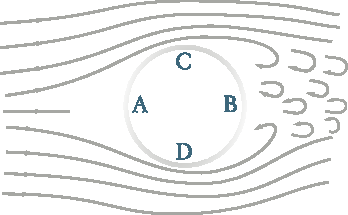
\includegraphics[scale=1.0]{figures/ch_09/fig_9_16.pdf}
			\caption[]{}
			\label{fig:9_16}
		\end{center}
	\end{minipage}
	\hspace{-0.0cm}
	\begin{minipage}[t]{0.5\linewidth}
		\begin{center}
			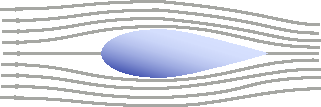
\includegraphics[scale=1.0]{figures/ch_09/fig_9_17.pdf}
			\caption[]{}
			\label{fig:9_17}
		\end{center}
	\end{minipage}
	\vspace{-0.5cm}
\end{figure}

%The ratio between the friction drag and the pressure drag is determined by the value of the Reynolds number~\eqref{eq:9_13}. Here, $l$ is a characteristic dimension of the body in question (for example, the radius for a spherical body), and $v$ is the velocity of the body relative to the fluid.

Hệ thức giữa lực cản do ma sát và lực cản do áp suất dược xác định bằng giá trị của số Reynolds~\eqref{eq:9_13}. Trong trường hợp này $l$ là một kích thước đặc trưng nào đó của vật (chẳng hạn, bán kính đối với vật có dạng cầu), $v$ là vận tốc của vật đối với chất lỏng.

%At small values of $\reynolds$, the main part is played by the friction drag, so that the pressure drag may be disregarded. The part of the pressure drag grows more and more with increasing $\reynolds$. At great values of $\reynolds$, pressure forces predominate in the drag.

Với $\reynolds$ nhỏ lực cản do ma sát đóng vai trò cơ bản, cho nên có thể không cần để ý tới lực cản do áp suất. Khi $\reynolds$ tăng vai trò của lực cản do áp suất sẽ càng lớn hơn. Với các giá trị $\reynolds$ lớn, các lực cản do áp suất sẽ vượt lực cản chính diện.

%When determining the nature of the forces acting on a body in a flow, the Reynolds number can be used as a similarity number (scale factor) in this case too. This circumstance is taken advantage of in modelling. For example, a model of an aeroplane will behave in a gas flow the same as the full-scale counterpart if in addition to geometrical similarity of the model and the aeroplane, the Reynolds number will also be equal for them.

Khi xác định đặc tính của các lực tác dụng lên vật trong dòng, số Reynolds có thể dùng làm tiêu chuẩn cho sự dồng dạng của các hiện tượng cả trong trường hợp này. Điều này được sử dụng trong việc mô hình hoá. Chẳng hạn, mô hình của máy bay sẽ hoạt động trong dòng khí theo cùng một cách như nguyên bản của nó, nếu ngoài sự đồng dạng hình học của mô hình và máy bay ra thì các số Reynolds đối với chúng cũng phải bằng nhau.

%\textbf{The Stokes Formula.} At small values of $\reynolds$, \ie, at low velocities [and small $l$'s, see \eqn{9_13}], the resistance of a medium is due virtually only to the friction forces. George Stokes (1819-1903) established that the drag force in this case is proportional to the dynamic viscosity $\eta$, the velocity $v$ of a body relative to the fluid, and the characteristic dimension of the body $l$, \ie $F\propto\eta lv$ (it is assumed that the distance from the body to the boundaries of the fluid, for example, to the walls of a vessel confining it, considerably exceeds the dimensions of the body). The proportionality constant depends on the form of the body. For a sphere, if we take its radius $r$ as the dimension $l$, the proportionality constant is $6\pi$. Hence, the drag force on a sphere in fluids at small velocities, according to the Stokes formula, is

\textbf{Công thức Stokes}. Với các $\reynolds$ nhỏ, nghĩa là với các vận tốc chuyển động không lớn [và các $l$ không lớn; xem \eqn{9_13}], sự cản của môi trường thực tế chỉ gây ra bởi các lực ma sát. Stokes đã thiết lập được là lực cản trong trường hợp này tỷ lệ đối với hệ số nhớt động lực học $\eta$, vận tốc chuyển động $v$ của vật đối với chất lỏng và kích thước đặc trưng $l$ của vật $F\propto\eta lv$ (giả thử là khoảng cách từ vật đến các biên của chất lỏng, chẳng hạn đến các thành bình, lớn hơn các kích thước của vật rất nhiều). Hệ số tỷ lệ phụ thuộc vào hình dạng của vật. Đối với một quả cầu nếu lấy bán kính $r$ của quả cầu làm $l$ thì hệ số tỷ lệ là bằng $6\pi$. Do đó lực cản chuyển động của quả cầu trong các chất lỏng với các vận tốc không lớn, theo công thức Stokes bằng 

\begin{equation}\label{eq:9_24}
	F = 6\pi\eta rv.
\end{equation}

%\textbf{Lift.} The viscosity of a fluid is of no significance for the appearance of a lift. Figure~\ref{fig:9_18} shows the streamlines when an ideal fluid flows around a half-cylinder. Owing to complete flowing around, the streamlines will be symmetrical relative to straight line CD. The pattern will not be symmetrical, however, relative to straight line AB. The streamlines are closer together near point C, therefore the pressure here will be lower than near point D, and the lift $\vec{P}$ appears. A lift appears similarly in a viscous fluid.

\textbf{Lực nâng.} Để làm xuất hiện lực nâng, thì tính nhớt của chất lỏng không có ý nghĩa quan trọng. Trên hình~\ref{fig:9_18} người ta trình bày các đường dòng khi chất lỏng lý tưởng chảy quanh một nửa hình trụ. Do chảy quanh hoàn toàn nên các đường dòng sẽ đối xứng với đường thẳng CD. Tuy nhiên đối với đường thẳng AB bức tranh sẽ không đối xứng. Các đường dòng sẽ dày đặc ở gần điểm C, vì vậy áp suất ở đây sẽ nhỏ hơn áp suất ở gần điểm D, và lực nâng $\vec{P}$ sẽ xuất hiện. Một cách tương tự, lực nâng sẽ xuất hiện cả trong chất lỏng nhớt.

\begin{figure}[!htb]
	\begin{minipage}[t]{0.5\linewidth}
		\begin{center}
			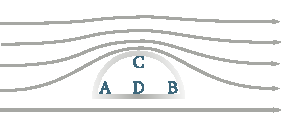
\includegraphics[scale=1.0]{figures/ch_09/fig_9_18.pdf}
			\caption[]{}
			\label{fig:9_18}
		\end{center}
	\end{minipage}
	\hspace{-0.1cm}
	\begin{minipage}[t]{0.5\linewidth}
		\begin{center}
			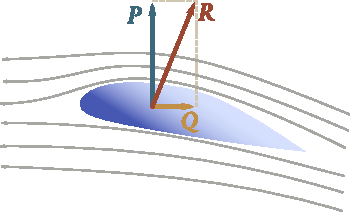
\includegraphics[scale=1.0]{figures/ch_09/fig_9_19.pdf}
			\caption[]{}
			\label{fig:9_19}
		\end{center}
	\end{minipage}
	\vspace{-0.5cm}
\end{figure}

%The force keeping an aeroplane in the air is the lift acting on its wings. The drag is harmful during the flight of an aeroplane. This is why the wings of an aeroplane and its fuselage are given a well streamlined shape. The profile of an aerofoil (wing) must also ensure an adequate lift. The profile shown in \fig{9_19}, found by the outstanding Russian scientist Nikolai Zhukovsky (1847-1921) is the optimal one for an aerofoil. The works of Zhukovsky and his pupil S. Chaplygin laid the foundation of modern aerodynamics. V. Lenin called Zhukovsky the father of Russian aviation. Zhukovsky, in particular, derived a formula for determining the lift that is the basis of all aerodynamic calculations of aeroplanes.

Lực nâng tác dụng lên cánh máy bay dùng làm lực đỡ máy bay trong không khí. Lực cản chính diện đóng vai trò có hại trong khi máy bay bay. Do đó người ta làm cho các cánh máy bay và thân của nó có dạng khá thuôn. Mặt cắt của cánh phải đồng thời đảm bảo một lực nâng đủ lớn. Mặt cắt do nhà bác học Nga vĩ đại Nikolai Zhukovsky (1847-1921) tìm được được trình bày trên \fig{9_19} là mặt cắt tối ưu cho cánh. Các công trình của Zhukovsky và học trò của ông là S. Chaplygin đã đặt nền móng cho môn khí động học hiện đại. V. Lenin đã gọi Zhukovsky là bố đẻ của ngành hàng không Nga. Cụ thể là Zhukovsky đã đưa ra công thức để xác định lực nâng là cơ sở của tất cả các phép tính toán về khí động học của các máy bay.
